\documentclass[10pt]{ctexart}
\usepackage{listings}
\usepackage{amsmath} 
\usepackage{amssymb} 
\usepackage{xcolor}
\usepackage{xeCJK}
\usepackage{fontspec}
\usepackage{titlesec}
\usepackage{titletoc}
\usepackage{setspace}
\usepackage{graphicx}
\usepackage{geometry}
\usepackage[T1]{fontenc}  
\usepackage{textcomp}
\usepackage{lmodern}
%\usepackage{caption}
\usepackage[justification=centering]{subcaption}
\usepackage[justification=centering]{caption}
\usepackage{tikz}
\usetikzlibrary{graphs}
\usepackage{amsfonts}
\usepackage[colorlinks,
            linkcolor=black,
            anchorcolor=black,
            citecolor=black]{hyperref}
\geometry{a4paper,scale=0.8}
\renewcommand\contentsname{Contents}
%\setmonofont[Mapping={}]{Monaco}    %英文引号之类的正常显示,相当于设置英文字体
%\setsansfont{Consolas} %设置英文字体 Monaco, Consolas,  Fantasque Sans Mono
%\setmainfont{Monaco} %设置英文字体
\setmonofont{Consolas}
% 定义可能使用到的颜色
%\setmainfont[BoldFont=SimHei]{SimSun}
\definecolor{CPPLight}  {HTML} {686868}
\definecolor{CPPSteel}  {HTML} {888888}
\definecolor{CPPDark}   {HTML} {262626}
\definecolor{CPPBlue}   {HTML} {4172A3}
\definecolor{CPPGreen}  {HTML} {487818}
\definecolor{CPPBrown}  {HTML} {A07040}
\definecolor{CPPRed}    {HTML} {AD4D3A}
\definecolor{CPPViolet} {HTML} {7040A0}
\definecolor{CPPGray}  {HTML} {B8B8B8}
\lstset{
    columns=fixed,       
    % numbers=left,                                        % 在左侧显示行号
    frame=none,                                          % 不显示背景边框
    backgroundcolor=\color[RGB]{245,245,244},            % 设定背景颜色
    keywordstyle=\color[RGB]{40,40,255},                 % 设定关键字颜色
    numberstyle=\small\color{darkgray},                  % 设定行号格式
    commentstyle=\it\color[RGB]{0,96,96},                % 设置代码注释的格式
    stringstyle=\rmfamily\slshape\color[RGB]{128,0,0},   % 设置字符串格式
    showstringspaces=false,                              % 不显示字符串中的空格
    language=c++,                                        % 设置语言
    morekeywords={alignas,continute,friend,register,true,alignof,decltype,goto,
    reinterpret_cast,try,asm,defult,if,return,typedef,auto,delete,inline,short,
    typeid,bool,do,int,signed,typename,break,double,long,sizeof,union,case,
    dynamic_cast,mutable,static,unsigned,catch,else,namespace,static_assert,using,
    char,enum,new,static_cast,virtual,char16_t,char32_t,explict,noexcept,struct,
    void,export,nullptr,switch,volatile,class,extern,operator,template,wchar_t,
    const,false,private,this,while,constexpr,float,protected,thread_local,
    const_cast,for,public,throw,std},
    emph={map,set,multimap,multiset,unordered_map,unordered_set,
    unordered_multiset,unordered_multimap,vector,string,list,deque,
    array,stack,forwared_list,iostream,memory,shared_ptr,unique_ptr,
    random,bitset,ostream,istream,cout,cin,endl,move,default_random_engine,
    uniform_int_distribution,iterator,algorithm,functional,bing,numeric,},
    emphstyle=\color{CPPViolet},
    basicstyle=\linespread{1}\small\fontspec{Consolas}\ttfamily,
    breaklines=true,
    %xleftmargin=1em,xrightmargin=1em, aboveskip=1em,
    % in the listings package configuration, try:  
    literate={"}{\textquotedbl}1,  
    tabsize=4, keepspaces=true
}
\CTEXoptions[today=old]
\title{Exercises 5}
\author{软件工程一班 \ 张逸松 57号}
\date{\today}

\begin{document}
    \maketitle
    \subsection*{6.1}
        \begin{itemize}
            \item [\textbf{a)}] It is partial ordering.
            \item [\textbf{b)}] It is not partial ordering. It is not transitive, not antisymmetric.
            \item [\textbf{c)}] It is partial ordering.
            \item [\textbf{d)}] It is partial ordering.
            \item [\textbf{e)}] It is not partial ordering. It is not transitive.
        \end{itemize}
    \subsection*{6.4}
        \begin{itemize}
            \item [\textbf{a)}] It is not partial ordering.
            \item [\textbf{b)}] It is partial ordering.
            \item [\textbf{c)}] It is not partial ordering.
        \end{itemize}
    \subsection*{6.5}
        It is partial ordering.
    \subsection*{6.12}
        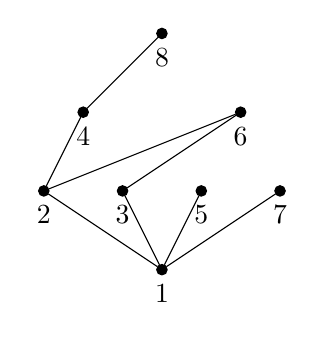
\begin{tikzpicture}
            \node (1) at (0, 0) [circle , draw, fill = black, label=below:$1$, scale = 0.4pt] {};
            \node (2) at (-1.5, 1) [circle , draw, fill = black, label=below:$2$, scale = 0.4pt] {};
            \node (3) at (-0.5, 1) [circle , draw, fill = black, label=below:$3$, scale = 0.4pt] {};
            \node (4) at (-1, 2) [circle , draw, fill = black, label=below:$4$, scale = 0.4pt] {};
            \node (5) at (0.5, 1) [circle , draw, fill = black, label=below:$5$, scale = 0.4pt] {};
            \node (6) at (1, 2) [circle , draw, fill = black, label=below:$6$, scale = 0.4pt] {};
            \node (7) at (1.5, 1) [circle , draw, fill = black, label=below:$7$, scale = 0.4pt] {};
            \node (8) at (0, 3) [circle , draw, fill = black, label=below:$8$, scale = 0.4pt] {};
            \draw [] (1) edge (2);
            \draw [] (1) edge (3);
            \draw [] (1) edge (5);
            \draw [] (1) edge (7);
            \draw [] (2) edge (4);
            \draw [] (2) edge (6);
            \draw [] (3) edge (6);
            \draw [] (4) edge (8);
        \end{tikzpicture}
        \quad
        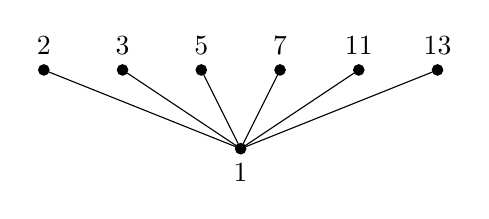
\begin{tikzpicture}
            \node (1) at (0, 0) [circle , draw, fill = black, label=below:$1$, scale = 0.4pt] {};
            \node (2) at (-2.5, 1) [circle , draw, fill = black, label=above:$2$, scale = 0.4pt] {};
            \node (3) at (-1.5, 1) [circle , draw, fill = black, label=above:$3$, scale = 0.4pt] {};
            \node (5) at (-0.5, 1) [circle , draw, fill = black, label=above:$5$, scale = 0.4pt] {};
            \node (7) at (0.5, 1) [circle , draw, fill = black, label=above:$7$, scale = 0.4pt] {};
            \node (11) at (1.5, 1) [circle , draw, fill = black, label=above:$11$, scale = 0.4pt] {};
            \node (13) at (2.5, 1) [circle , draw, fill = black, label=above:$13$, scale = 0.4pt] {};
            \draw [] (1) edge (2);
            \draw [] (1) edge (3);
            \draw [] (1) edge (5);
            \draw [] (1) edge (7);
            \draw [] (1) edge (11);
            \draw [] (1) edge (13);
        \end{tikzpicture}
        \quad
        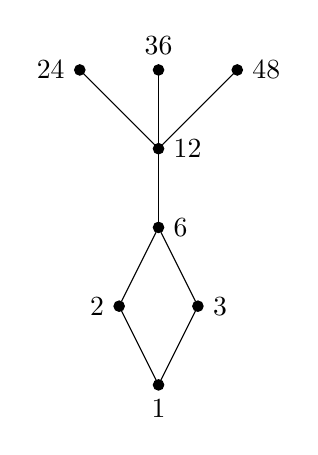
\begin{tikzpicture}
            \node (1) at (0, 0) [circle , draw, fill = black, label=below:$1$, scale = 0.4pt] {};
            \node (2) at (-0.5, 1) [circle , draw, fill = black, label=left:$2$, scale = 0.4pt] {};
            \node (3) at (0.5, 1) [circle , draw, fill = black, label=right:$3$, scale = 0.4pt] {};
            \node (6) at (0, 2) [circle , draw, fill = black, label=right:$6$, scale = 0.4pt] {};
            \node (12) at (0, 3) [circle , draw, fill = black, label=right:$12$, scale = 0.4pt] {};
            \node (24) at (-1, 4) [circle , draw, fill = black, label=left:$24$, scale = 0.4pt] {};
            \node (36) at (0, 4) [circle , draw, fill = black, label=above:$36$, scale = 0.4pt] {};
            \node (48) at (1, 4) [circle , draw, fill = black, label=right:$48$, scale = 0.4pt] {};
            \draw [] (1) edge (2);
            \draw [] (1) edge (3);
            \draw [] (2) edge (6);
            \draw [] (3) edge (6);
            \draw [] (6) edge (12);
            \draw [] (12) edge (24);
            \draw [] (12) edge (36);
            \draw [] (12) edge (48);
        \end{tikzpicture}
        \quad
        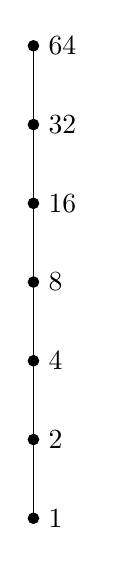
\begin{tikzpicture}
            \node (1) at (0, 0) [circle , draw, fill = black, label=right:$1$, scale = 0.4pt] {};
            \node (2) at (0, 1) [circle , draw, fill = black, label=right:$2$, scale = 0.4pt] {};
            \node (4) at (0, 2) [circle , draw, fill = black, label=right:$4$, scale = 0.4pt] {};
            \node (8) at (0, 3) [circle , draw, fill = black, label=right:$8$, scale = 0.4pt] {};
            \node (16) at (0, 4) [circle , draw, fill = black, label=right:$16$, scale = 0.4pt] {};
            \node (32) at (0, 5) [circle , draw, fill = black, label=right:$32$, scale = 0.4pt] {};
            \node (64) at (0, 6) [circle , draw, fill = black, label=right:$64$, scale = 0.4pt] {};
            \draw [] (1) edge (2);
            \draw [] (2) edge (4);
            \draw [] (4) edge (8);
            \draw [] (8) edge (16);
            \draw [] (16) edge (32);
            \draw [] (32) edge (64);
        \end{tikzpicture}
\end{document}